\section{Model finalny i raport wynikow}

\subsection{Cel i zakres analizy modelu}
W tej sekcji dokumentujemy finalny model klasyfikacji \texttt{human} vs \texttt{bot},
z naciskiem na:
\begin{itemize}
  \item jakie dane i cechy weszly do treningu,
  \item jak wykonano podzial na trening i test,
  \item jak przeprowadzono walidacje i ewaluacje,
  \item na ile wyniki odpowiadaja rzeczywistemu dzialaniu systemu.
\end{itemize}

\subsection{Konfiguracja modelu finalnego}
Finalna wersja modelu to drzewo decyzyjne trenowane na cechach behawioralnych:
\begin{itemize}
  \item algorytm: \texttt{DecisionTreeClassifier},
  \item parametry okna: \texttt{window\_size = 120}, \texttt{stride = 80},
  \item hiperparametry: \texttt{max\_depth = 12}, \texttt{min\_samples\_leaf = 2},
  \item \texttt{class\_weight = balanced},
  \item \texttt{feature\_set = behavioral} (bez cech srodowiskowych).
\end{itemize}

\subsection{Jakie dane weszly do modelu}
\subsubsection{Poziom surowy}
Wejsciem sa sesje zapisane w PostgreSQL (\texttt{sessions}, \texttt{raw\_events}),
z etykieta referencyjna \texttt{true\_label} nadana przez operatora.
Kazde okno zawiera uporzadkowany po czasie fragment zachowania, a nie pojedynczy event.

\subsubsection{Poziom cech}
Z okna eventow budowane sa cechy opisujace:
\begin{itemize}
  \item dynamike ruchu kursora: \texttt{speed\_*}, \texttt{acc\_*}, \texttt{jerk\_*},
  \item geometrie toru: \texttt{path\_length}, \texttt{path\_efficiency}, \texttt{curvature\_*},
  \item mikrozachowania: \texttt{micro\_pause\_count}, \texttt{correction\_rhythm}, \texttt{overshoot\_count},
  \item wzorzec klikniec i scrolla: \texttt{click\_interval\_*}, \texttt{hover\_before\_click\_mean},
  \texttt{scroll\_velocity\_*},
  \item entropie sekwencji: \texttt{event\_type\_entropy}, \texttt{unique\_event\_types}.
\end{itemize}

W finalnym modelu swiadomie pominieto cechy srodowiskowe (np. \texttt{viewport\_area}),
zeby ograniczyc ryzyko sztucznego zawyzania wyniku przez data leakage.

\subsection{Dobor zmiennych: proces i uzasadnienie}
\subsubsection{Przestrzen kandydacka i finalny wybor}
Proces startowal od pelnego slownika cech wyliczanego przez pipeline
(\texttt{FEATURE\_COLUMNS}) opisany w Tabeli~\ref{tab:feature-dictionary}.
W praktyce byly to:
\begin{itemize}
  \item 43 cechy kandydackie lacznie,
  \item 7 cech srodowiskowych,
  \item 36 cech behawioralnych.
\end{itemize}

Do finalnego modelu weszly cechy behawioralne
(\texttt{feature\_set=behavioral}), natomiast cechy srodowiskowe zostaly
wylaczone z trenowania drzewa.

\subsubsection{Kryteria doboru zmiennych}
Selekcja byla oparta o trzy kryteria:
\begin{itemize}
  \item \textbf{odpornosc na leakage}: odciecie sygnalow typu
  \texttt{viewport\_area} i \texttt{screen\_area}, ktore moga rozdzielac klasy
  na skroty, bez realnej analizy zachowania,
  \item \textbf{zwiazek z mikrodynamika ruchu}: preferencja dla cech opisujacych
  kinetyke i geometrie toru (\texttt{acc\_*}, \texttt{speed\_*}, \texttt{curvature\_*}),
  \item \textbf{interpretowalnosc}: drzewo z tak dobranym zbiorem cech daje
  reguly decyzyjne, ktore mozna odczytac i wyjasnic.
\end{itemize}

\subsubsection{Co oznacza ten wybor w praktyce}
Model finalny klasyfikuje sesje glownie na podstawie \emph{jak} porusza sie kursor
i jak wyglada rytm interakcji, a nie \emph{na czym} sesja jest wykonywana.
To zwieksza wiarygodnosc demonstracji, bo decyzja nie wynika z jednego artefaktu
srodowiskowego, tylko z profilu zachowania.

\subsection{Podzial train/test i walidacja}
\subsubsection{Strategia podzialu}
Podzial zostal wykonany przez \texttt{GroupShuffleSplit} z \texttt{test\_size=0.25}
i grupowaniem po \texttt{session\_id}. To kluczowe, bo:
\begin{itemize}
  \item okna z tej samej sesji nie trafiaja jednoczesnie do train i test,
  \item test sprawdza uogolnienie na nieznane sesje, a nie tylko nieznane okna.
\end{itemize}

\subsubsection{Co oznaczaja liczby w praktyce}
Z raportu metryk treningowych (Tabela~\ref{tab:train-metrics} i
Tabela~\ref{tab:train-cm}) wynika, ze zbior testowy mial 136 okien
(\texttt{TN+FP+FN+TP = 74+1+6+55}).
W ewaluacji aktywnego modelu analizowano 644 okna i 202 sesje
(Tabela~\ref{tab:eval-operational}).

\subsubsection{Typ walidacji}
W MVP uzyto pojedynczego hold-out splitu grupowego (jedna probka walidacyjna).
To dobre rozwiazanie demonstracyjne, ale nie zastepuje pelnej walidacji krzyzowej
np. \texttt{GroupKFold}.

\subsection{Metryki ilosciowe}
% Auto-generated by raport/scripts/refresh_model_assets.ps1
% Source timestamp: 20260515_173306

\subsubsection{Metryki z treningu (hold-out, GroupShuffleSplit)}
\begin{table}[H]
  \centering
  \begin{tabular}{l c}
    \toprule
    Metryka & Wartosc \\
    \midrule
    Precision & 0.9821 \\
    Recall & 0.9016 \\
    F1-score & 0.9402 \\
    ROC-AUC & 0.9442 \\
    False Positive Rate (human) & 0.0133 \\
    \bottomrule
  \end{tabular}
  \caption{Metryki modelu na zbiorze testowym podczas treningu}
  \label{tab:train-metrics}
\end{table}

\begin{table}[H]
  \centering
  \begin{tabular}{l c}
    \toprule
    Element & Wartosc \\
    \midrule
    TN & 74 \\
    FP & 1 \\
    FN & 6 \\
    TP & 55 \\
    \bottomrule
  \end{tabular}
  \caption{Confusion matrix (trening)}
  \label{tab:train-cm}
\end{table}
\subsubsection{Metryki ewaluacyjne (aktywny model)}
\begin{table}[H]
  \centering
  \begin{tabular}{l c}
    \toprule
    Metryka & Wartosc \\
    \midrule
    Precision & 0.9940 \\
    Recall & 0.9651 \\
    F1-score & 0.9794 \\
    ROC-AUC & 0.9815 \\
    False Positive Rate (human) & 0.0021 \\
    \bottomrule
  \end{tabular}
  \caption{Metryki z raportu ewaluacyjnego}
  \label{tab:eval-metrics}
\end{table}

\begin{table}[H]
  \centering
  \begin{tabular}{l c}
    \toprule
    Wskaznik & Wartosc \\
    \midrule
    Liczba probek & 644 \\
    Liczba sesji & 202 \\
    Avg events to detect bot & 122.2574 \\
    Median events to detect bot & 120.0000 \\
    Detection delay count & 101 \\
    Unseen bot recall count & 0 \\
    \bottomrule
  \end{tabular}
  \caption{Statystyki operacyjne ewaluacji}
  \label{tab:eval-operational}
\end{table}


Wyniki z testu hold-out (Tabela~\ref{tab:train-metrics}) sa mocne
(\texttt{F1=0.9402}, \texttt{ROC-AUC=0.9442}) przy niskim
\texttt{false positive rate} dla klasy \texttt{human} (\texttt{0.0133}).

\subsection{Wizualizacje modelu}
\begin{figure}[H]
  \centering
  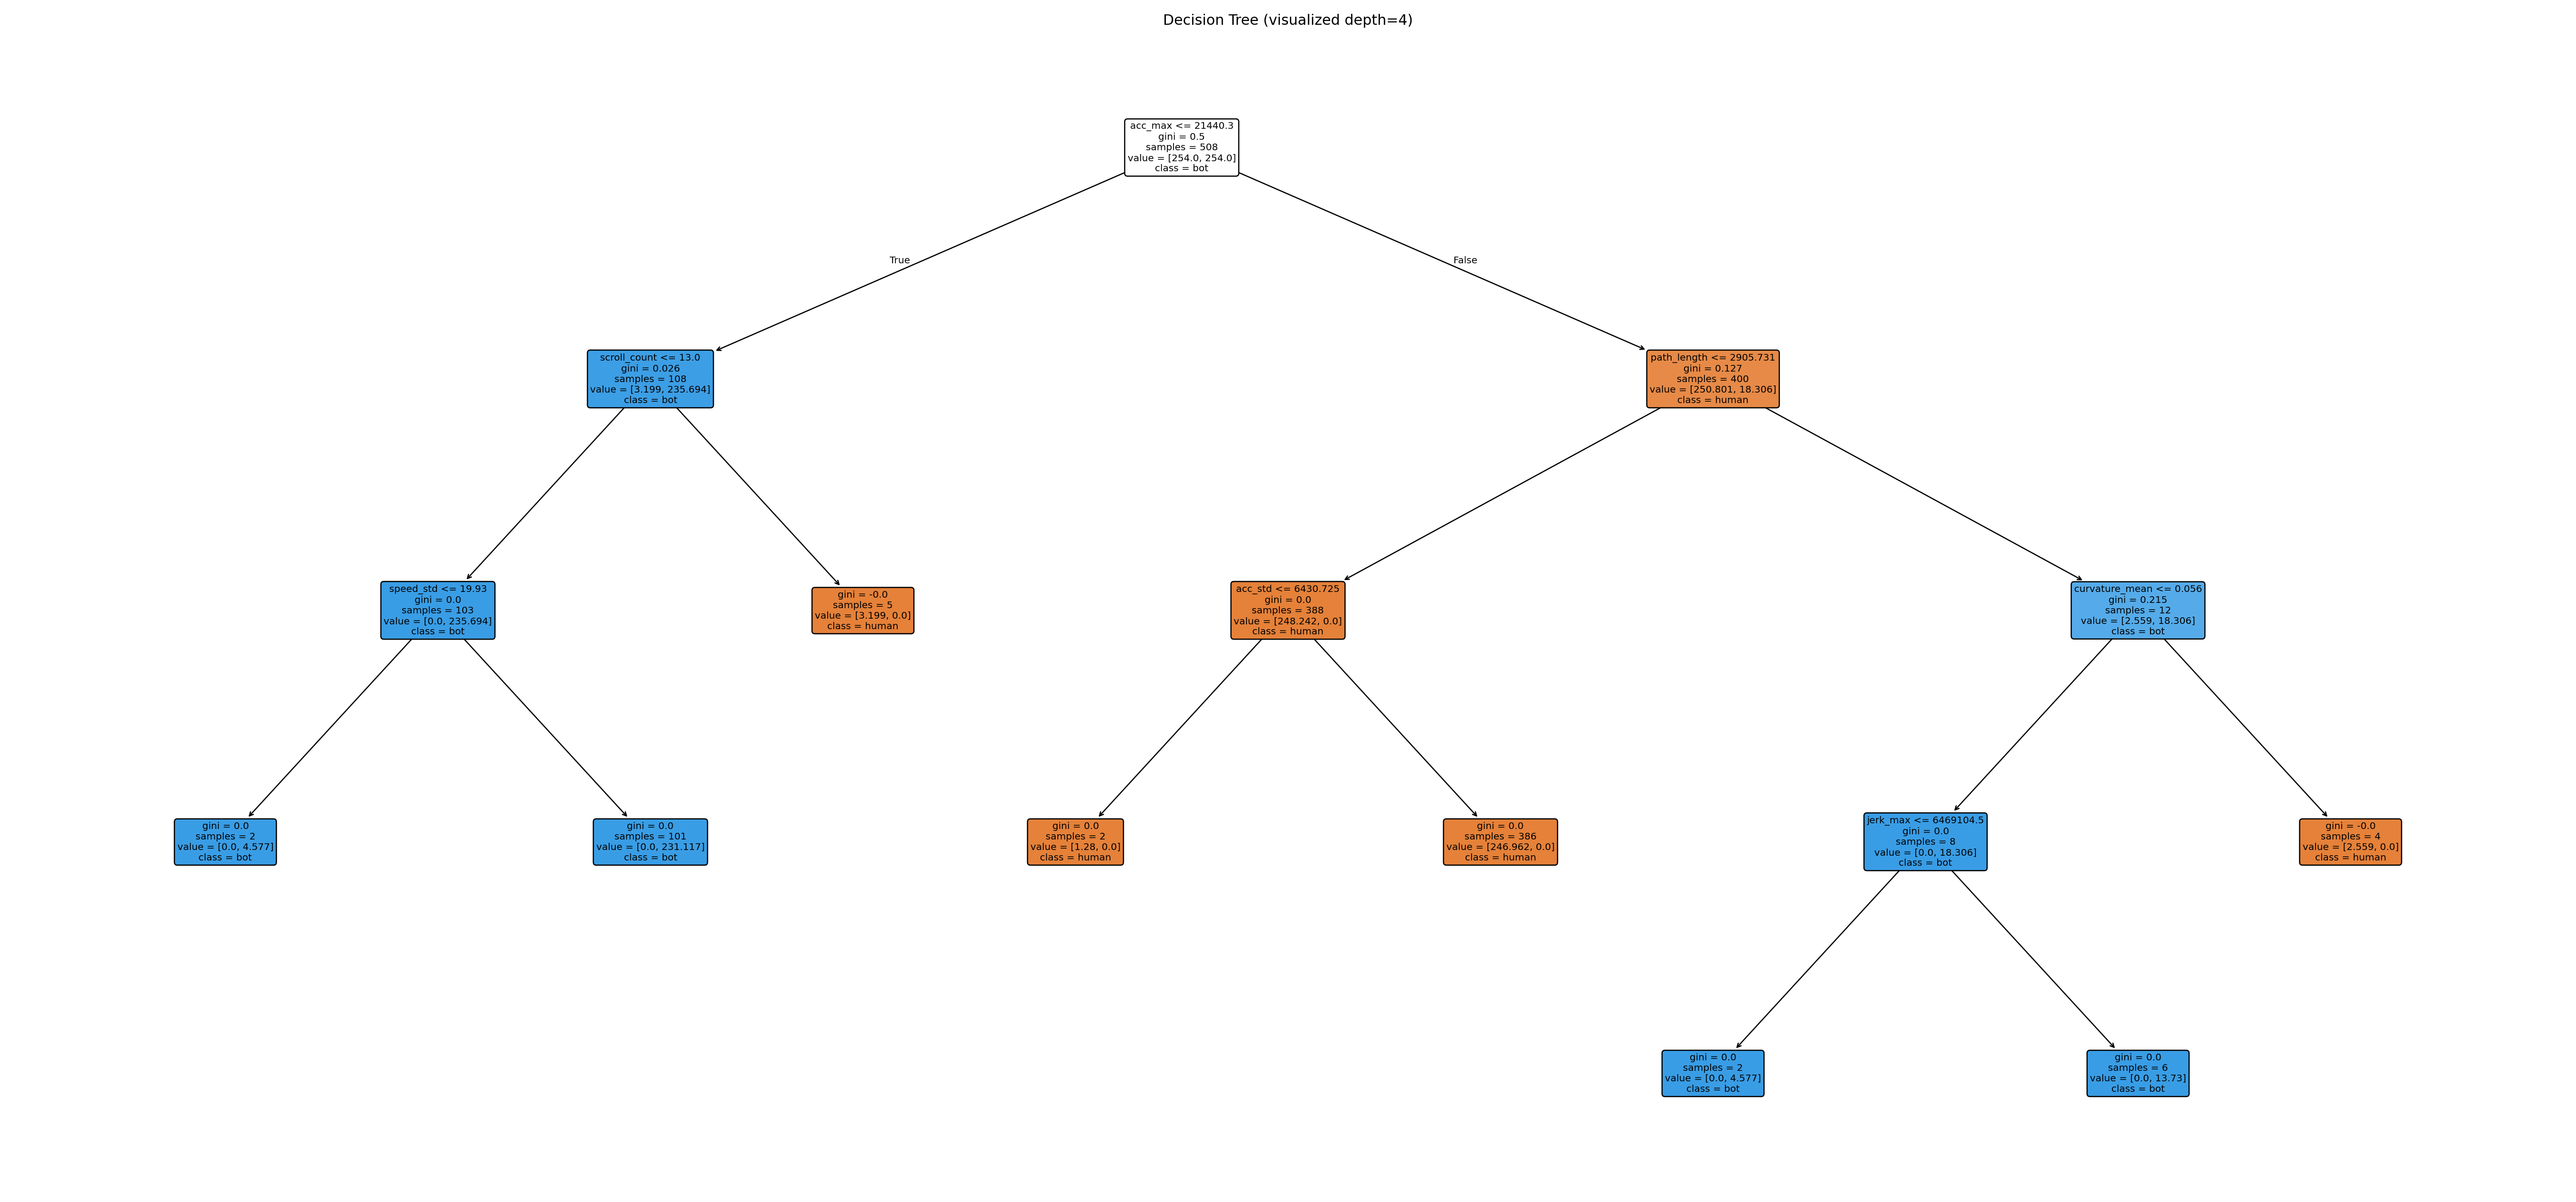
\includegraphics[width=0.72\textwidth]{figures/model/decision_tree_20260515_173306.png}
  \caption{Diagram drzewa decyzyjnego (warstwy najwyzszego poziomu)}
  \label{fig:model-tree}
\end{figure}

\begin{figure}[H]
  \centering
  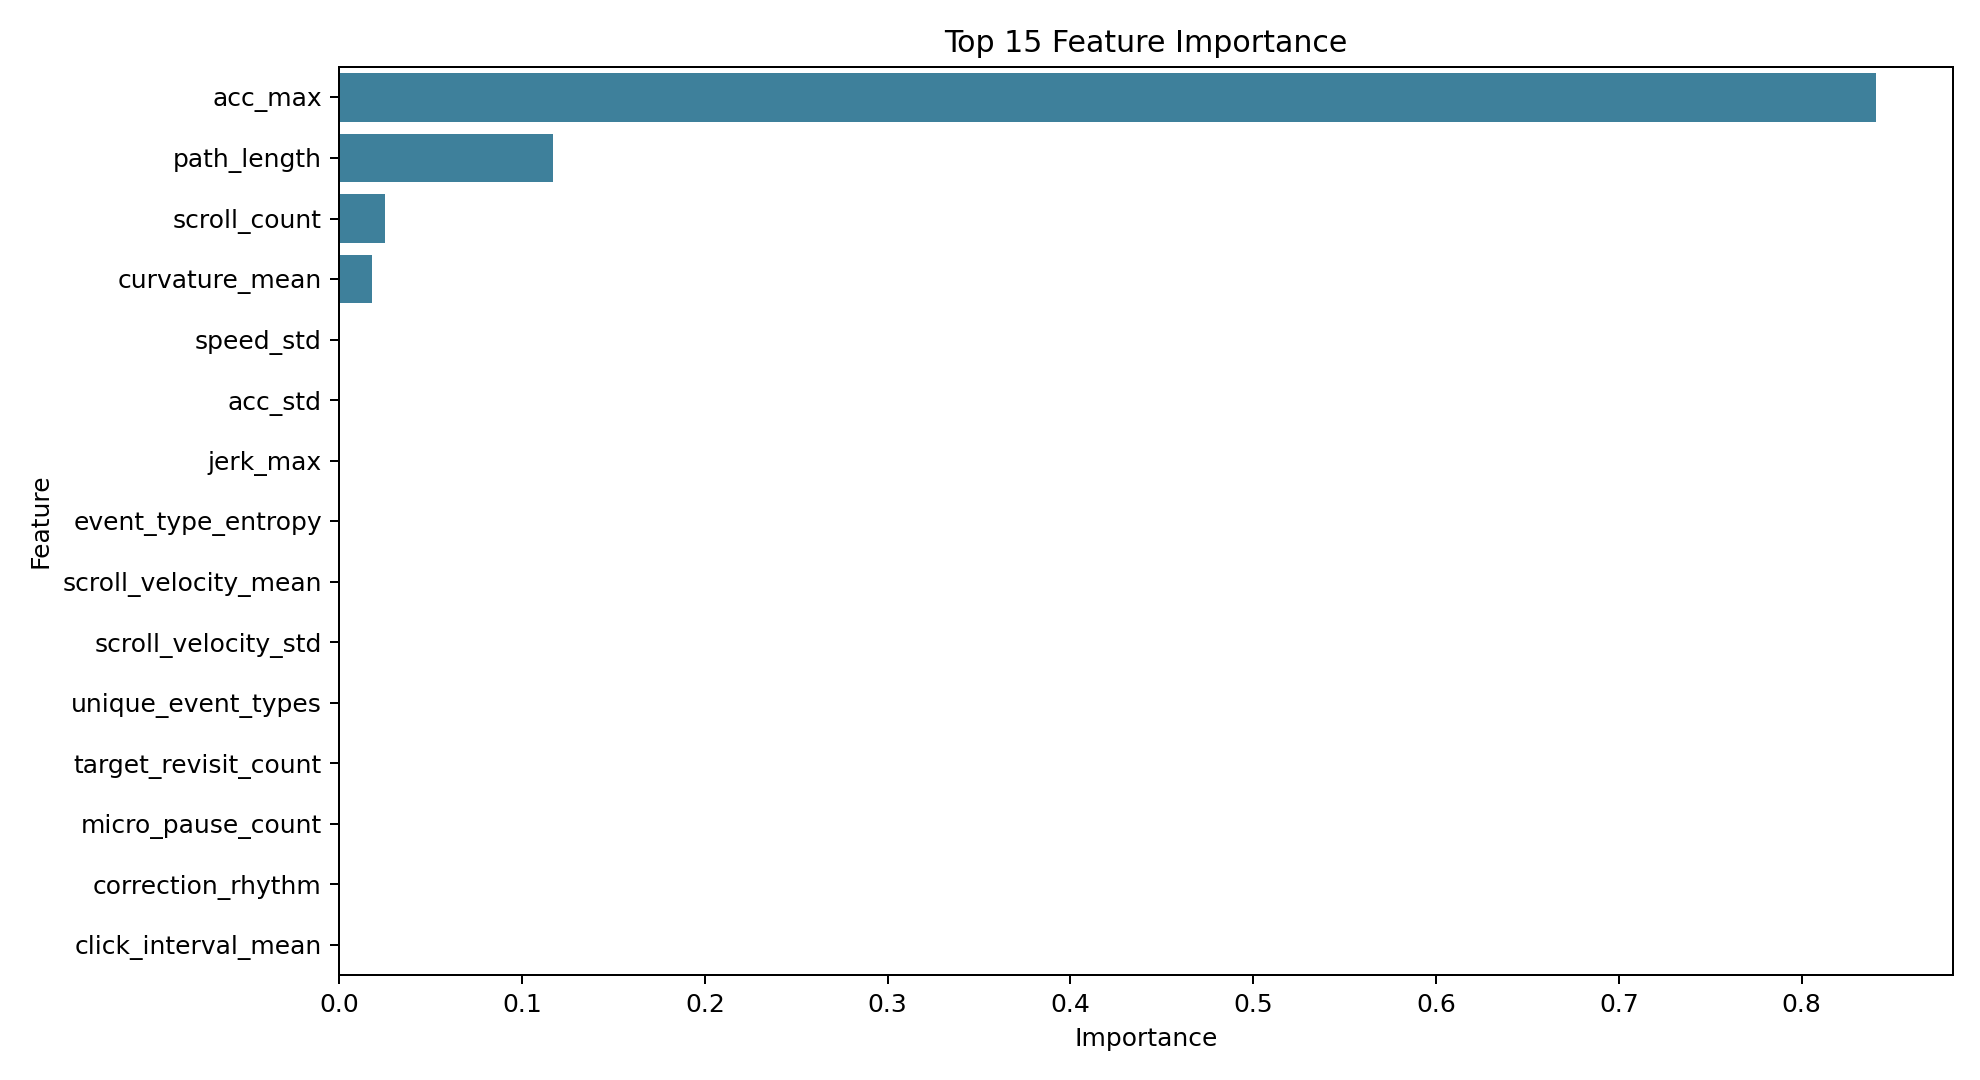
\includegraphics[width=0.8\textwidth]{figures/model/decision_tree_feature_importance_20260515_173306.png}
  \caption{Waznosc cech (feature importance) dla modelu finalnego}
  \label{fig:model-importance}
\end{figure}

\begin{figure}[H]
  \centering
  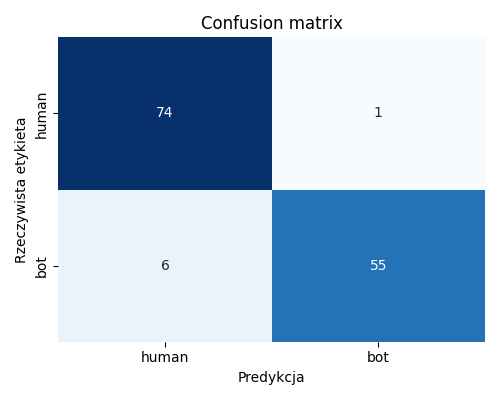
\includegraphics[width=0.45\textwidth]{figures/model/confusion_matrix_20260515_173306.png}
  \hfill
  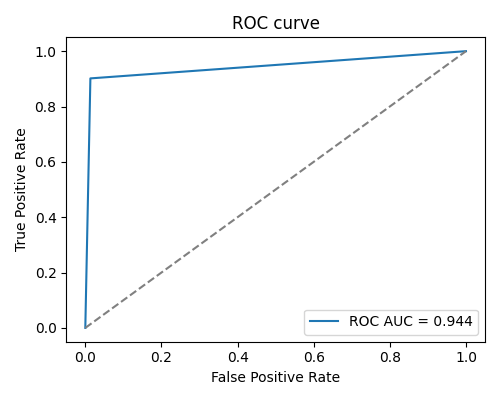
\includegraphics[width=0.45\textwidth]{figures/model/roc_20260515_173306.png}
  \caption{Confusion matrix oraz ROC dla zbioru testowego w treningu}
  \label{fig:train-cm-roc}
\end{figure}

\begin{figure}[H]
  \centering
  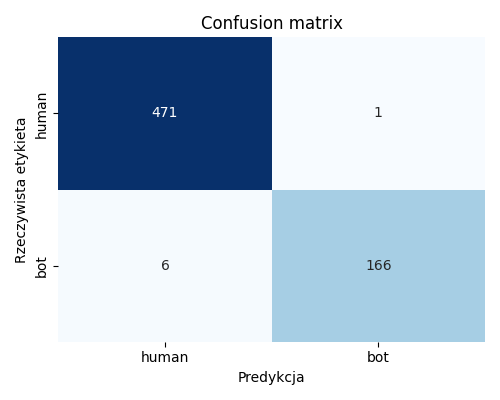
\includegraphics[width=0.45\textwidth]{figures/model/eval_confusion_matrix.png}
  \hfill
  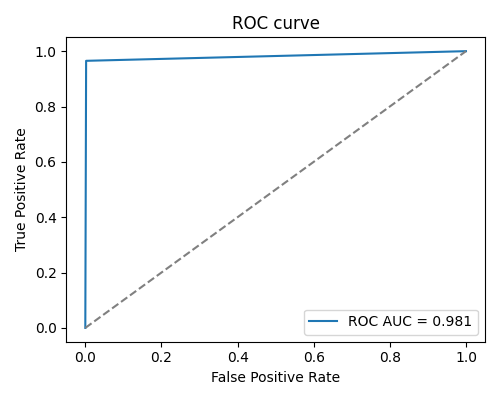
\includegraphics[width=0.45\textwidth]{figures/model/eval_roc.png}
  \caption{Confusion matrix oraz ROC w ewaluacji aktywnego modelu}
  \label{fig:eval-cm-roc}
\end{figure}

\subsection{Interpretacja: co model rzeczywiscie robi}
Rysunek~\ref{fig:model-tree} pokazuje, ze model jest interpretowalny i mozna
odczytac jawne warunki decyzji. Rysunek~\ref{fig:model-importance} potwierdza,
ze dominujaca cecha to nadal \texttt{acc\_max}, a kolejne sygnaly (np. \texttt{path\_length},
\texttt{event\_type\_entropy}) sa uzupelniajace.

\subsubsection{Struktura decyzyjna drzewa: interpretacja warstw}
Na podstawie Rysunku~\ref{fig:model-tree} i pelnych regul mozna odczytac
nastepujaca logike:
\begin{itemize}
  \item \textbf{Wezel glowny (\texttt{acc\_max})}: pierwszy podzial oddziela
  sesje o niskich i wysokich pikach przyspieszenia kursora.
  \item \textbf{Galaz niskiego \texttt{acc\_max}}: kolejne warunki
  \texttt{scroll\_count} i \texttt{speed\_std} prowadza glownie do klasy \texttt{bot}.
  Intuicyjnie: ruch jest bardziej wygladzony i mniej impulsywny.
  \item \textbf{Galaz wysokiego \texttt{acc\_max}}: podzialy po
  \texttt{path\_length} i \texttt{acc\_std} czesciej prowadza do klasy \texttt{human},
  bo odzwierciedlaja bardziej zrywny i korekcyjny tor ruchu.
  \item \textbf{Wezly glebsze} (\texttt{curvature\_mean}, \texttt{jerk\_max})
  doprecyzowuja decyzje dla przypadkow granicznych, gdzie sama dynamika pierwszego
  rzedu nie wystarcza.
\end{itemize}

\subsubsection{Jak czytac diagram waznosci cech}
Rysunek~\ref{fig:model-importance} przedstawia waznosci typu impurity-based
(spadek nieczystosci wezlow, Gini). Interpretacja:
\begin{itemize}
  \item wysoka waznosc \texttt{acc\_max} oznacza, ze ta cecha najczesciej daje
  najwiekszy przyrost informacji przy podzialach,
  \item niezerowa rola \texttt{path\_length} i \texttt{event\_type\_entropy}
  pokazuje, ze model korzysta takze z geometrii toru i roznorodnosci sekwencji eventow,
  \item niska waznosc wielu cech nie oznacza, ze sa globalnie niepotrzebne; oznacza,
  ze w aktualnej probie byly rzadziej wybierane jako najlepszy podzial.
\end{itemize}

\subsubsection{Znaczenie operacyjne (co to oznacza dla detekcji)}
Struktura drzewa jest spojna z celem systemu:
\begin{itemize}
  \item sesje o zbyt gladkiej mikrodynamice sa przesuwane w strone \texttt{bot},
  \item sesje z naturalnymi korektami i zrywami ruchu sa przesuwane w strone \texttt{human},
  \item policy engine otrzymuje wynik oparty o zachowanie, a nie o pojedynczy artefakt
  srodowiskowy.
\end{itemize}

\subsection{Reguly klasyfikacji (fragment)}
Model pozostaje interpretowalny -- mozna odczytac reguly decyzyjne:
\begin{lstlisting}[style=reportcode,caption={Przykladowy fragment regul drzewa decyzyjnego},label={lst:tree-rules-fragment}]
|--- acc_max <= 21440.2998
|   |--- scroll_count <= 13.0000
|   |   |--- speed_std <= 19.9304 -> class: bot
|--- acc_max > 21440.2998
|   |--- path_length <= 2905.7310
|   |   |--- acc_std > 6430.7249 -> class: human
\end{lstlisting}

Listing~\ref{lst:tree-rules-fragment} jest bezposrednim dopelnieniem
Rysunku~\ref{fig:model-tree}: po podziale na \texttt{acc\_max} drzewo
doprecyzowuje decyzje przez \texttt{scroll\_count}, \texttt{speed\_std},
\texttt{path\_length} i \texttt{acc\_std}. Taka sekwencja warunkow jest
czytelna biznesowo i latwa do audytu.

\subsection{Czy ewaluacja jest spojna z rzeczywistoscia?}
\subsubsection{Co jest spojne}
\begin{itemize}
  \item Hold-out test (Rysunek~\ref{fig:train-cm-roc}) i metryki z Tabeli~\ref{tab:train-metrics}
  pokazuja, ze model dobrze odroznia klasy na nieznanych sesjach testowych.
  \item Metryka \texttt{detection delay} (Tabela~\ref{tab:eval-operational}) daje praktyczny sygnal,
  po ilu eventach system zwykle wykrywa bota.
\end{itemize}

\subsubsection{Gdzie jest ryzyko przeszacowania}
\begin{itemize}
  \item Ewaluacja aktywnego modelu (Tabela~\ref{tab:eval-metrics}, Rysunek~\ref{fig:eval-cm-roc})
  liczona jest na calym zbiorze oznaczonych okien, wiec zawiera rowniez dane
  wykorzystane do treningu.
  \item To oznacza, ze wyniki ewaluacyjne sa bardziej optymistyczne niz hold-out
  i nie powinny byc jedynym kryterium oceny generalizacji.
\end{itemize}

\subsubsection{Najwazniejsze ograniczenie obecnego raportu}
W Tabeli~\ref{tab:eval-operational} \texttt{unseen\_bot\_recall} ma \texttt{count=0},
czyli w aktualnym zestawie nie ma osobnej, niewidzianej rodziny botow do twardego testu OOD.
Dlatego aktualny raport dobrze opisuje zachowanie modelu \emph{w ramach obecnej dystrybucji},
ale nie zamyka tematu odpornosci na nowe klasy botow.

\subsection{Threats to validity}
Ponizej wskazano glowne ryzyka interpretacyjne wynikow:
\begin{itemize}
  \item \textbf{Internal validity}: mimo wykluczenia czesci cech srodowiskowych z podzialow drzewa,
  pozostaje ryzyko, ze model wykorzystuje sygnaly specyficzne dla aktualnego UI i sposobu testowania.
  \item \textbf{Construct validity}: etykieta \texttt{human} opiera sie na recznym oznaczaniu sesji,
  co jest praktyczne, ale moze zawierac szum (np. sesja czlowieka z nienaturalnym rytmem).
  \item \textbf{External validity}: dane pochodza glownie z lokalnego srodowiska (localhost),
  ograniczonej liczby urzadzen/przegladarek i kontrolowanych scenariuszy.
  \item \textbf{Conclusion validity}: zastosowano pojedynczy hold-out split grupowy,
  bez wielokrotnej walidacji (\texttt{GroupKFold}) i bez przedzialow ufnosci metryk.
  \item \textbf{OOD validity}: brak niezaleznej rodziny botow w metryce \texttt{unseen\_bot\_recall}
  (\texttt{count=0}) utrudnia twarda ocene odpornosci na nowe techniki automatyzacji.
\end{itemize}

Wniosek praktyczny: metryki sa mocne dla aktualnej dystrybucji danych,
ale produkcyjna pewnosc wymaga dalszego rozszerzania zbioru i walidacji wielokrotnej.

\subsection{Wniosek koncowy}
Model finalny jest mocny i interpretowalny na aktualnym zbiorze (patrz
Tabela~\ref{tab:train-metrics} i Rysunek~\ref{fig:model-tree}),
jednak dla pelnej zgodnosci z warunkami produkcyjnymi potrzebuje kolejnego kroku:
oddzielnego testu na niewidzianych scenariuszach botowych oraz walidacji wielokrotnej
na poziomie sesji.

